\documentclass[12pt]{article}
\usepackage[margin=1in]{geometry}
\setlength{\parindent}{0pt}
\usepackage{graphicx}
\usepackage{amsmath}
\usepackage{amssymb}
\usepackage{multicol}

\begin{document}

\title{Latent Space Planning Notes}
\author{}
\date{}

\maketitle

\begin{abstract}
My notes on papers for latent space planning.
\end{abstract}

\section{Efficient Planning in a Compact Latent Action Space}
They introduce Trajectory Autoencoding Planning (TAP) for planning in the learned compact latent action space. Sequence of actions are mapped into a discrete latent space. This reduces the number of variables the model considers during planning. 

TAP reasons about the trajectory as a whole because every latent represents L sequence of actions. This scales well with higher dimensions as the latent space is smaller and more structured than the raw action space.

The latent is learned using a state conditioned (gets the first state as input) VQ-VAE, so the latent space is discrete. Causal transformers are used for the encoder, decoder and the prior policy. The policy is trained to maximize the expected return (g) and uses Monte carlo Sampling to estimate the gradient.

\newpage
\section{Learning Predictive Representations for Deformable Objects Using Contrastive Estimation}
In this paper they learn the latent dynamics of a deformable object (rope and cloth) using contrastive estimation (InfoNCE Loss). The latent model and the forward model are trained jointly.

Planning is done using a model predictive where several actions are sampled and are run through the forward model from the current \(\mathbf{z}_{t}\). Then choose action theta produces \(\hat{\mathbf{z}}_{t+1}\) closest to the goal embedding (l2-distance).

Contrastive forward models outperforms all baselines because they can generalize well as the latent space is task driven. If MSE Loss was used, reconstruction would be the priority and hence lighting and other sorts of noise will be fit, whereas, CFM regularizes to encode the latent space with task relevant information by not fitting the noise. Baselines like autoencoders and PlaNet fail to generalize effectively with DR, as they focus on reconstructing fine-grained details irrelevant to the task (e.g., lighting and color).

Domain randomization in sim facilitated Sim-to-Real.
\begin{figure}[ht]
    \centering
    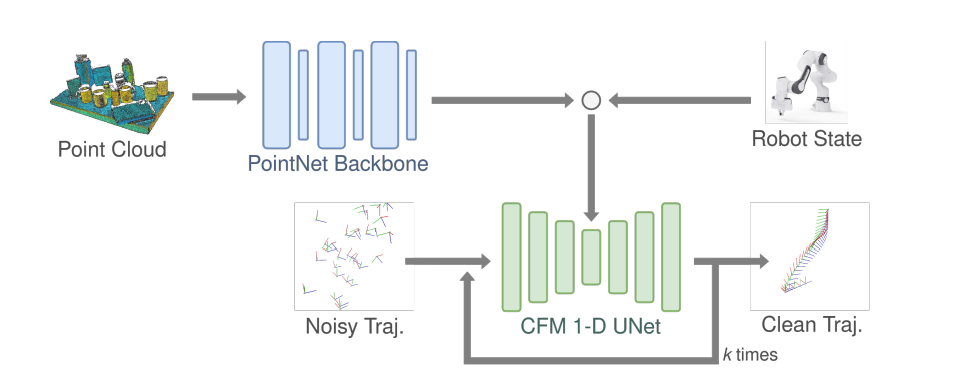
\includegraphics[width=0.8\textwidth]{/home/devesh/Notes/Papers/Latent Space Planning/1.png}
    \caption{}
    \label{fig:latent_dynamics}
\end{figure}

\subsection{InfoNCE Loss}
InfoNCE (Information Noise-Contrastive Estimation) Loss is used to learn representations by maximizing the mutual information between the input and the output. It contrasts the positive pairs (correct pairs) against negative pairs (incorrect pairs) to ensure that the learned representations are informative and discriminative. The loss is defined as:

\[
\mathcal{L}_{\text{InfoNCE}} = -\mathbb{E} \left[ \log \frac{h(\hat{\mathbf{z}}_{t+1}, \mathbf{z}_{t+1})}{\sum_{i=1}^{k} h(\hat{\mathbf{z}}_{t+1}, \tilde{\mathbf{z}}_i)} \right]
\]

where \(h(\cdot, \cdot)\) is a similarity function, \(\hat{\mathbf{z}}_{t+1}\) and \(\mathbf{z}_{t+1}\) are the latent representations of the positive pair, and \(\tilde{\mathbf{z}}_i\) are the latent representations of the negative samples.

\newpage
\section{Physics-Informed Neural ODE (PINODE): Embedding Physics into Models using Collocation Points}
\begin{multicols}{2}
\[
\frac{d}{dt} x(t) = f(x(t))
\]

\[
\frac{d}{dt} z(t) = h(z(t))
\]

\[
z(0) = \psi^{-1}(x(0))
\]

\[
z(T) = z(0) + \int_{0}^{T} h(z(t)) \, dt
\]

\[
x(T) = \psi(z(T))
\]
The decoder, encoder are \(\psi , \phi\) respectively. Latent dynamics evolve according to \(h\).
\end{multicols}

\[
\mathcal{L}_{\text{data}}^{\theta} = \frac{1}{2\sigma^2} \sum_{i=1}^{k} \left[ \omega_1 \sum_{j=1}^{p} \left\| x_i(t_j) - \psi_{\theta} (\phi_{\theta} (x_i(t_j))) \right\|^2 + \omega_2 \sum_{j=1}^{p} \left\| \psi_{\theta} \left( \phi_{\theta} (x_i(t_1)) + \int_{t_1}^{t_j} h(z(t)) \, dt \right) - x_i(t_j) \right\|^2 \right]
\]

\begin{multicols}{2}
\((\bar{x}, f(\bar{x}))\) are collocation points sampled from the space to incorporate physics through loss fn. 
\[
\frac{d z(x(t))}{d t} = \frac{d z}{d x} \frac{d x}{d t} = \nabla \phi(x(t))^T f(x(t))
\]

\[
\frac{d z(x(t))}{d t} = h(\phi(x(t)))
\]

\[
h(\phi(x(t))) = \nabla \phi(x)^T f(x)
\]
\end{multicols}

\[
\mathcal{L}_{\text{physics}}^{\theta} = \sum_{i=1}^{N} \left[ \frac{\omega_3}{N} \left\| h_{\theta} (\phi_{\theta} (\bar{x}_i)) - \nabla \phi_{\theta} (\bar{x}_i) f(\bar{x}_i) \right\|^2 + \frac{\omega_4}{N} \left\| \bar{x}_i - \psi_{\theta} (\phi_{\theta} (\bar{x}_i)) \right\|^2 \right]
\]
\begin{figure}[ht]
    \centering
    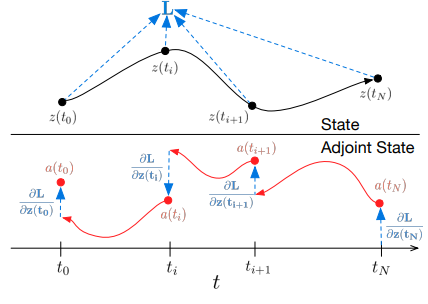
\includegraphics[width=0.8\textwidth]{/home/devesh/Notes/Papers/Latent Space Planning/2.png}
    \caption{}
    \label{fig:pinode}
\end{figure}

\newpage

\end{document}